\section{System Overview}

The system essentially consists of a mobile manipulator (Mirte Master) tasked with
autonomously exploring an indoor environment (the robotics lab), identifying and localizing objects, distinguishing between electronics and other objects, and sorting these objects accordingly. The task can be broken down as follows:

The main task of the robot can be broken down into sub-tasks which then fit into specific niches of the entire system architecture. \textbf{Motion planning}, \textbf{perception} and \textbf{navigation}. \texttt{\{numref\}Figure \{number\} \textless fig-task\_bins\textgreater } showcases this idea.

\begin{figure}[!htbp]
\centering
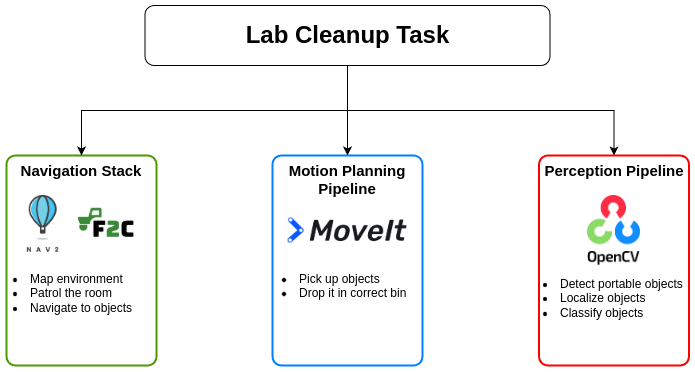
\includegraphics[width=0.7\linewidth]{figures/task_bins-6a576b2f1c55451f442d86eee45bd124.png}
\end{figure}

The scope of our investigation includes how different perception(classification) and navigation(mapping and patrolling) approaches influence the performance of the whole system. The highest performing combination of approaches is then chosen for use in the respective subsystems.

\subsection{System level strategy}

The system level strategy consists of how the robot behaves in each scenario that it will find itself. The tasks described above are used as a guideline to construct the full system level strategy. The standard in robotics for such navigation and perception heavy tasks is to use a global behavior tree that describes how the robot ought to behave in certain situations. This system level architecture as shown in \texttt{\{numref\}Figure \{number\} \textless fig-global\_tree\textgreater } is also used here to describe and execute the cleaning strategy.

\begin{figure}[!htbp]
\centering
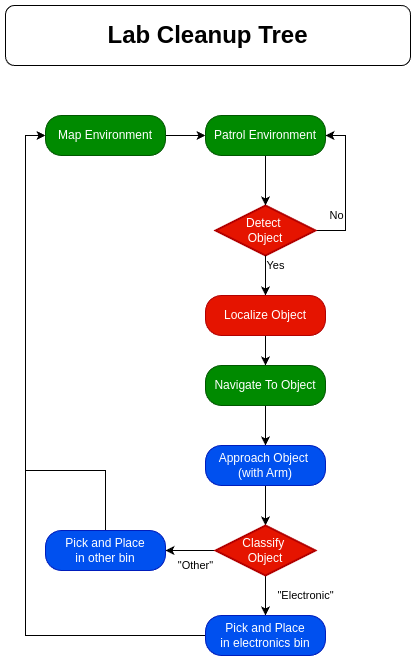
\includegraphics[width=0.7\linewidth]{figures/global_tree-eeb791198186b710db5720ebe0f0af19.png}
\end{figure}

\subsection{Navigation}

The navigation stack of this robot, powered by nav2 and fields2cover, executes three main tasks:

\begin{itemize}
\item Mapping
\item Patrolling
\item Object Approach
\end{itemize}

\subsubsection{Mapping}

Before the robot can navigate properly through the environment and ensure proper coverage, this environment must first be known. Thats where mapping approaches come in handy. Several advanced and specialized mapping approaches exist already, but in this paper only three are considered. Frontier based mapping, \{2\}, \{3\}. These were chosen through a combination of novelty and frequent application in similar contexts. Once the environment is mapped \{sufficiently\} the robot is allowed to navigate the space and propagate its behavior further down the tree.

\begin{quote}
Add ros2 bag playback
\end{quote}

\subsubsection{Patrolling}

Two categories of coverage strategies are implemented:

\textbf{Systematic Navigation:} The environment is traversed using a structured pattern to ensure complete coverage. These approaches are often called coverage methods and paired with decomposition methods discussed in the theory section

\textbf{Reactive Navigation}: The robot dynamically traverses and selects exploration targets based on frontier regions or detected objects, prioritizing areas of high information gain.

\begin{quote}
iets meer over coverage planning.
\end{quote}

\textbf{Free space:}
The ROS framework allows for integration with a lot of modular software packages. throughout the years this has given rise to many universally applied packages, Nav2 is such a case.
Using Nav2 the Global Costmap can be used to extrapolate the free space for the robot to move in.

\subsection{Perception}

Perception is responsible for object detection, classification and spatial localization. For this study we limited the object detection and localization approaches to two. A \textbf{2D detection and depth projection} approach, and 3D segmentation with \textbf{point cloud clustering}.
As for classification methods, this study evaluates a classical cv approach, aswell as a classification model based approach.

objects are categorized into:

\begin{enumerate}
\item Graspable vs non-graspable
\item Electronics vs non-electronics
\end{enumerate}

\begin{quote}
iets meer over classification.
\end{quote}